\documentclass[12pt]{extarticle}

\usepackage[utf8]{inputenc}
\usepackage[T1]{fontenc}
\usepackage{lmodern}
\usepackage{graphicx}
\usepackage{color}
\usepackage{hyperref}
\usepackage{amsmath}
\usepackage{amsfonts}
\usepackage{epstopdf}
\usepackage[table]{xcolor}
\usepackage[a4paper, total={6in, 10in}]{geometry}
\usepackage{enumitem}
\usepackage[export]{adjustbox}
\usepackage{algorithm2e}
\usepackage{adjustbox}

\graphicspath{ {./Figures/} }

\begin{document}

{\Large Andrew Sivaprakasam | Warm-Up 2 Write-up}

GitHub Repo: \url{https://github.com/sivaprakasaman/Numerical_Methods_BME/} 

\section{Solving a Nonlinear Single Equation}
\stepcounter{subsection}


\subsection{Bisection Method Thought Exercise | Task List 1-A}

\begin{enumerate}
\item A, B, and C demonstrate cases where there may or may not be a root between $f(x_1)$ and $f(x_m)$ when their product is greater than zero. 
**\textbf{Note:} when I drew these, I accidentally put $x_u$ instead of $x_m$.
\item A and B also demonstrate that there may be multiple roots between $x_1$ and $x_u$ when their product is greater than zero.
\\
\begin{center}
\includegraphics[width = .45\textwidth]{pic_1}
\includegraphics[width = .45\textwidth]{pic_2}
\end{center}

\item Bisection Method Flowchart (see code for implementation):
\begin{center}
\textit{flowchart from codingalpha.com}
\includegraphics[width = .6\textwidth]{bisect_flow}
\end{center}
\end{enumerate}

\newpage
\subsection{Newton's Method | Task List 1-B}
\begin{enumerate}
\item Below is a flowchart demonstrating Newton's Method:
\begin{center}
\textit{flowchart from codingalpha.com}
\includegraphics[width = .6\textwidth]{newton_flow}
\end{center}
\item Here is a table showing iteration $k$, $x_k$, and $\epsilon$ for the first root-finding problem. $\epsilon$ was set to $10^{-6}$.

\begin{center}
\begin{adjustbox}{width=.45\columnwidth,center}
\begin{tabular}{|r|r|r|}
\hline
\multicolumn{1}{|l|}{$k$} & \multicolumn{1}{l|}{$x_k$} & \multicolumn{1}{l|}{$\epsilon$} \\ \hline
0 & 1 & \multicolumn{1}{l|}{Inf} \\ \hline
1 & 0.687116367041199 & 0.455357560912301 \\ \hline
2 & 0.479569647933555 & 0.432777011643571 \\ \hline
3 & 0.342752246343126 & 0.399172880849518 \\ \hline
4 & 0.253830851560911 & 0.350317521433663 \\ \hline
5 & 0.19792929482791 & 0.282431950164854 \\ \hline
6 & 0.165573528412162 & 0.195416300697569 \\ \hline
7 & 0.150538921218223 & 0.099871894074121 \\ \hline
8 & 0.146628975172691 & 0.026665575756273 \\ \hline
9 & 0.146360742307274 & 0.001832683144324 \\ \hline
10 & 0.146359504721027 & 8.46E-06 \\ \hline
\end{tabular}
\end{adjustbox}
\label{}

\end{center}

\item Here is a table for the minimization problem, also showing iteration $k$, $x_k$, and $\epsilon$. $\epsilon$ was set to $10^{-6}$.
\begin{center}
\begin{adjustbox}{width=.45\columnwidth,center}
\begin{tabular}{|r|r|r|}
\hline
\multicolumn{1}{|l|}{$k$} & \multicolumn{1}{l|}{$x_k$} & \multicolumn{1}{l|}{$\epsilon$} \\ \hline
0 & 1 & \multicolumn{1}{l|}{Inf} \\ \hline
1 & 0.950777558639313 & 0.051770722724179 \\ \hline
2 & 0.947754440621915 & 0.003189769298696 \\ \hline
3 & 0.947747133558387 & 7.71E-06 \\ \hline
\end{tabular}
\label{}
\end{adjustbox}
\end{center}
\end{enumerate}

\newpage
\subsection{Comparison of Algorithms | Task List 1-C}
Wall-clock runtime analysis demonstrates, in the cases provided, that the bisection method performs faster than the Newton Method in the top two figures. HOWEVER, this absolutely does not mean Bisection Method is better than Newton's Method. In fact, the bisection requires more iterations to converge to a solution within error $\epsilon$ as seen in the bottom figure. The bisection method converges linearly while Newton's Method converges quadratically.
\\ \\
\textit{The limiting factor in this case is likely the fact that Newton's Method requires the evaluation of a derivative prior to iterating, which computationally takes a good bit of time. 
}
\begin{center}
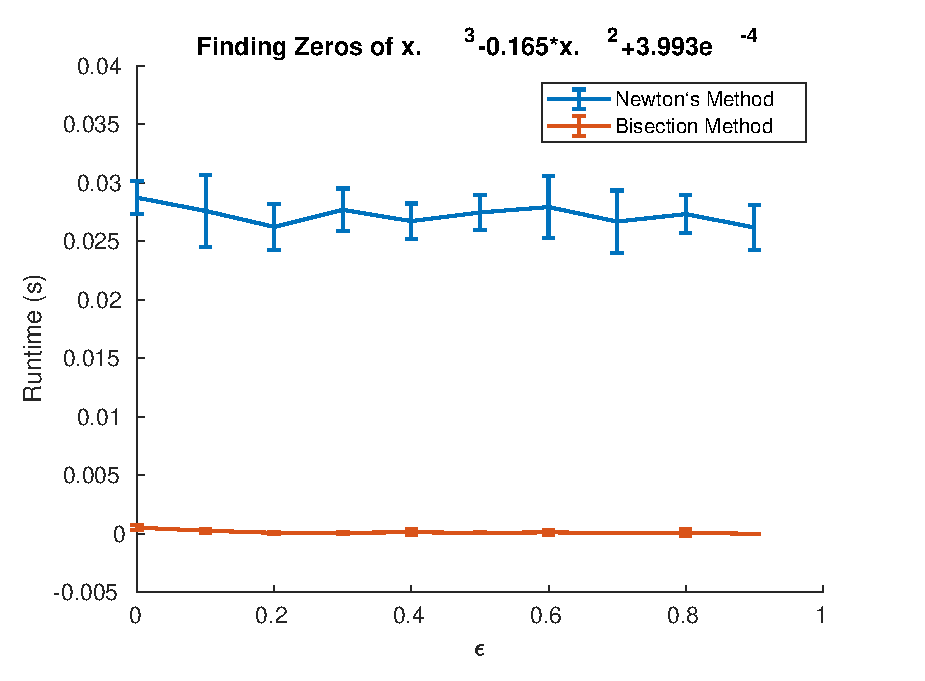
\includegraphics[width = .49\textwidth]{runtime1}
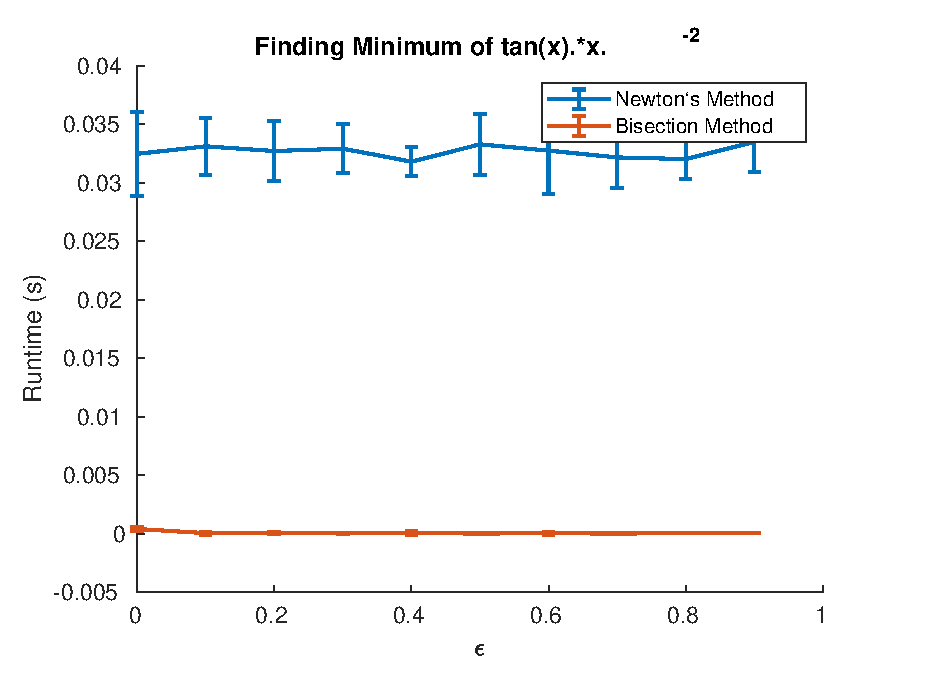
\includegraphics[width = .49\textwidth]{runtime2}\\
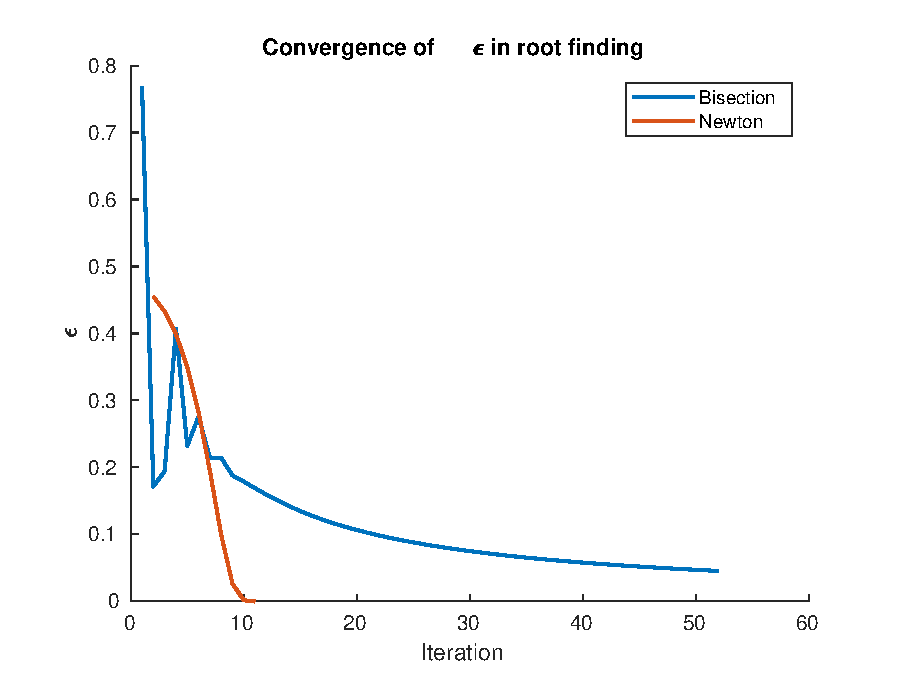
\includegraphics[width = .55\textwidth]{convergence}
\end{center}

\newpage
\section{Runge-Kutta Methods}
\begin{enumerate}

\item Euler's Method (RK1), RK2, and RK4 estimations of the solution to the ODE $y^{\prime} = -y$ were compared to the analytical solution (black). Notably, the RK4 estimation was closest followed by RK2 and Euler's Method. See code for implementations.
\begin{center}
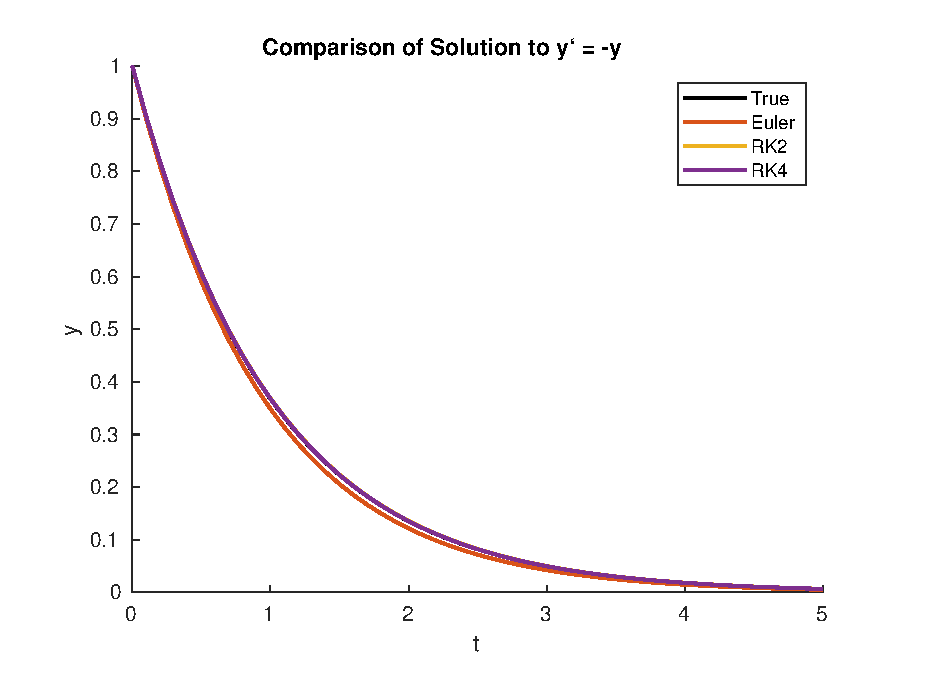
\includegraphics[width = .47\textwidth]{comp1}
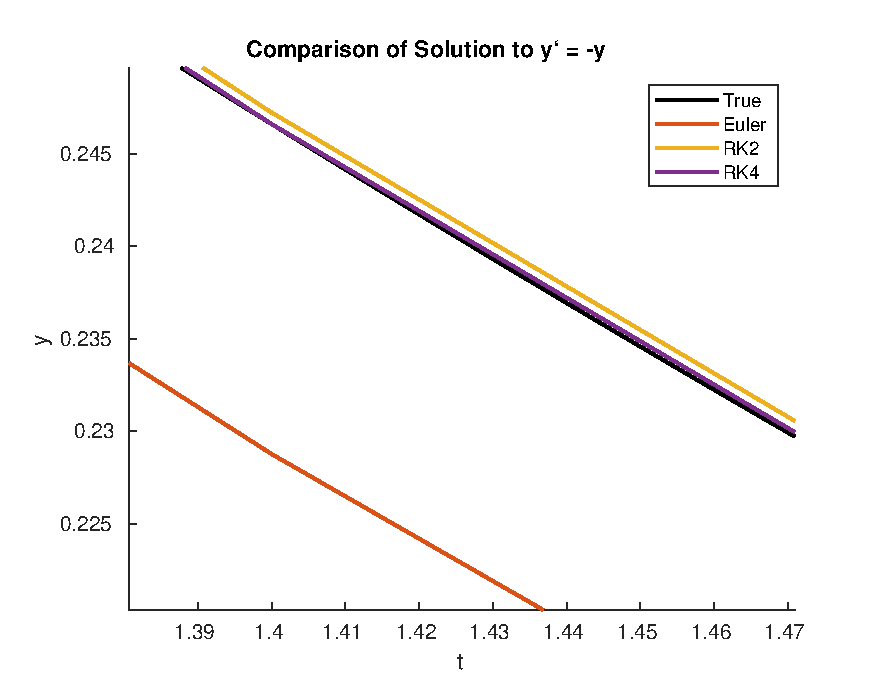
\includegraphics[width = .43\textwidth]{zoomed_in}
\end{center}

\item Similar findings were observed in the approximations for the ODE $y^{\prime} + 2y = 2-e^{-4t}$. 
\begin{center}
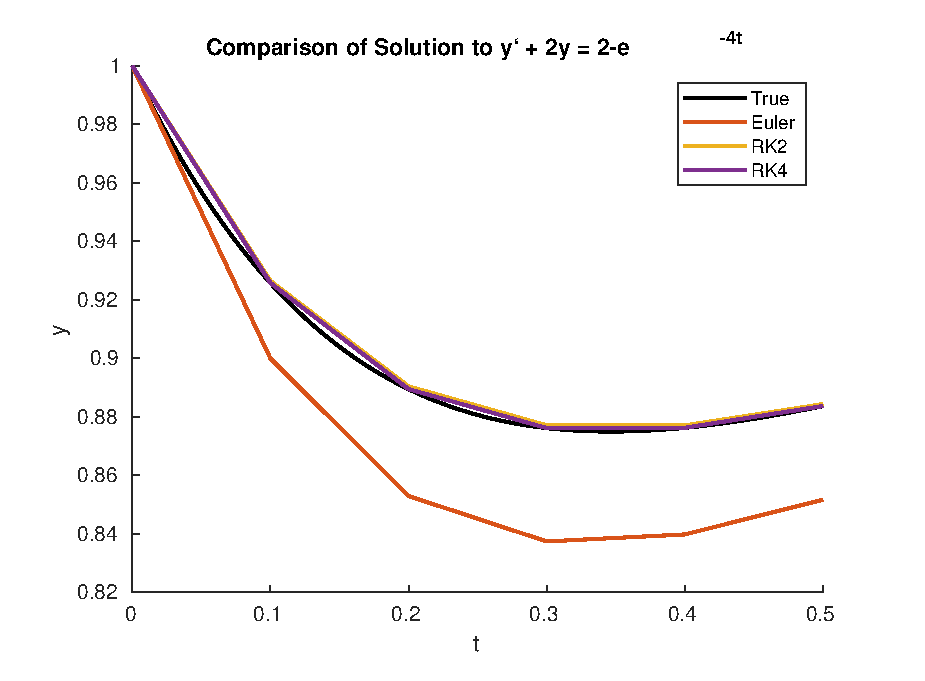
\includegraphics[width = .65\textwidth]{comp2}
\end{center}
\end{enumerate}


\section{Nelder-Mead Optimization Algorithm}
\begin{itemize}
\item The Nelder-Mead algorithm can primarily be used when trying to determine the minimums presented in an $n$-dimensional function. This might be particularly useful in mapping the lowest point of a 3D map or in \textit{non-linear optimization problems} such as Rosenbrock's Function. Nelder-Mead can also be used when the derivative of the function is not known, for example in a black-box type problem where a system must be perturbed in order to quantify a response.

\item Using the \verb|fminsearch| function, I was able to ascertain that the minimum of the Rosenbrock function is $[1,1]$.
\end{itemize}

\end{document}